\section{Background}

\subsection{Spike-by-Spike Neural Networks}
\label{sec:sbs}

Technically, SbS is a spiking neural network approach based on a
generative probabilistic model. It iteratively finds an estimate of
its input probability distribution $p(s)$ (i.e. the probability of
input node $s$ to stochastically send a spike) by its latent variables
via $r(s) = \sum_i h(i) W(s|i)$. 
where $\vec{h}$ is an inference
population composed of a group of neurons that compete with each
other. An inference population sees only the spikes $s_t$ (i.e. the
index identifying the input neuron $s$ which generated that spike at
time $t$) produced by its input neurons, not the underlying input
probability distribution $p(s)$ itself. By counting the spikes
arriving at a group of SbS neurons, $p(s)$ is estimated by
$\hat{p}(s) = 1/T \sum_t \delta_{s,s^t}$ after $T$ spikes have been
observed in total. The goal is to generate an internal representation
$r(s)$ from the string of incoming spikes $s_t$ such that the negative
logarithm of the likelihood
$L = C - \sum_\mu \sum_s \hat{p}_\mu(s) log\left( r_\mu(s) \right)$ is
minimized. $C$ is a constant which is independent of the internal
representation $r_\mu(s)$ and $\mu$ denotes one input pattern from an
ensemble of input patterns. Applying a multiplicative gradient descent
method on $L$, an algorithm for iteratively updating $h_\mu(i)$ with
every observed input spike $s_t$ could be derived
\cite{ernst2007efficient}
  \begin{eqnarray} \label{eq:sbs_update}
  h_\mu^{new}(i) = \frac{1}{1+\epsilon} \left(h_\mu(i) + \epsilon \frac{h_\mu(i) W(s_t|i) }{\sum_j h_\mu(j) W(s_t|j)} \right) 
  \end{eqnarray}
  where $\epsilon$ is a parameter that also controls the strength of sparseness of the distribution of latent variables $h_\mu(i)$. Furthermore, $L$ can also be used to derive online and batch learning rules for optimizing the weights $W(s|i)$. The interested reader is referred to \cite{ernst2007efficient} for a more detailed exposition.

  \REVIEW{ From a practical point of view, SbS provides a mechanism to obtain a sparse representation of input patterns. Given a set of
    training samples $\{x_\eta\}$, it learns weights ($W$), that allow
    to express the input patterns as a linear sparse non-negative combination
    of features.  During inference, it provides a mechanism for expressing
    each test input $x_\mu$ as $x_\mu \approx W\, h_\mu$ where all
    entries are non-negative.

    The inference procedure consists in generating indices $s_t$
    distributed according to a categorical distribution of the input pattern
    $s_t \sim \mathrm{Categorical}(x_{\mu}(0), x_{\mu}(1), ..,
    x_{\mu}(N-1))$. Starting with a random $h$ and executing
    iteratively \mbox{\Equ{eq:sbs_update}} the SbS algorithms finds
    $h_{\mu}$. The fundamental concept of SbS can be extended from vector to matrix
    inputs. In this case, the linear operation $W\, h_\mu$ can be replaced by a
    convolution to obtain a convolutional SbS layer. A detailed description of the SbS algorithm is presented in the supplementary material of this paper.}

%%%% This is added by Yarib, please review it
%%%%\subsection{Parallelization in SbS networks}
\subsection{\REVIEW{Basic Network Overview}}

\begin{figure}[!t]
	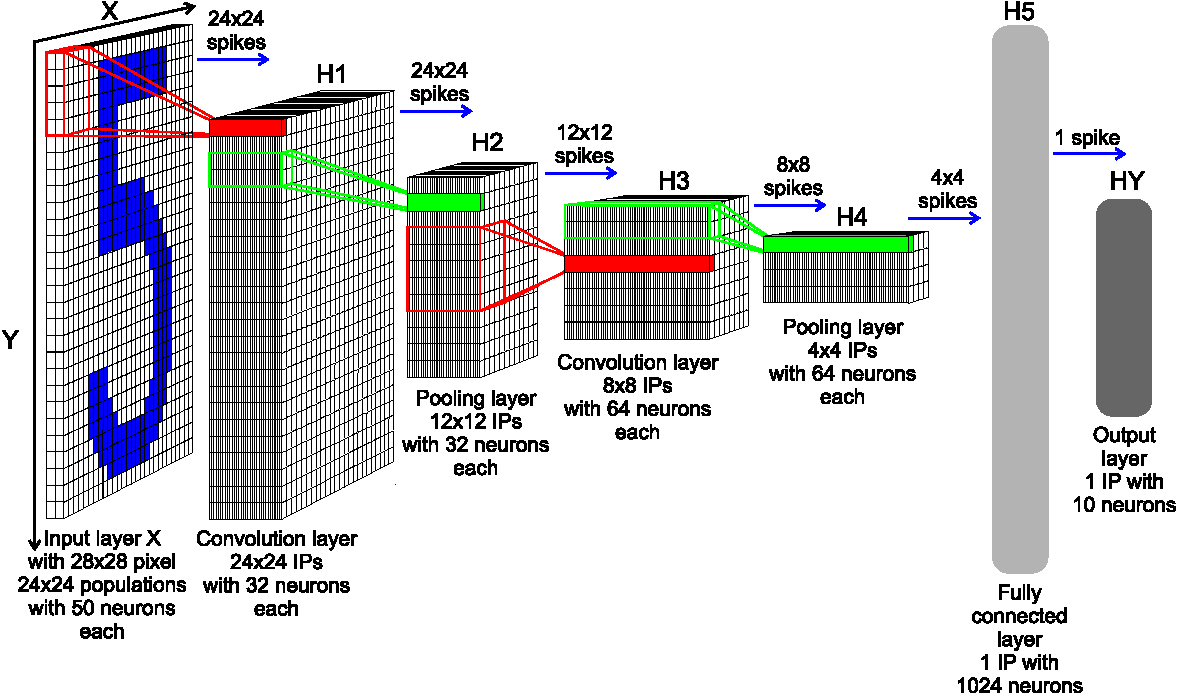
\includegraphics[width=\columnwidth]{../figures/sbs_network.pdf}
	\caption{SbS network architecture for handwritten digit classification task.}
	\label{fig:sbs_network}
\end{figure}


\begin{table}[!t]\centering
	\caption{SbS network architecture for handwritten digit classification task.}
	\label{tab:sbs_network}
	\scriptsize
	\begin{tabular}{lrrrrrrr}\toprule
		&\multicolumn{3}{c}{\textbf{Layer size}} & &\multicolumn{2}{c}{\textbf{Kernel size}} \\\cmidrule{2-4}\cmidrule{6-7}
		\textbf{Layer} ($H^l$) &$N_X$ &$N_Y$ &$N_H$ & &$K_X$ &$K_Y$ \\\midrule
		Input ($HX$) &28 &28 &2 & &- &- \\
		Convolution ($H1$) &24 &24 &32 & &5 &5 \\
		Pooling ($H2$) &12 &12 &32 & &2 &2 \\
		Convolution ($H3$) &8 &8 &64 & &5 &5 \\
		Pooling ($H4$) &4 &4 &64 & &2 &2 \\
		Fully connected ($H5$) &1 &1 &1024 & &4 &4 \\
		Output ($HY$) &1 &1 &10 & &1 &1 \\
		\bottomrule
	\end{tabular}
\end{table}

\begin{algorithm}[h!]
	\label{alg:sbs}
	\caption{SbS algorithm.}
	
	\begin{algorithmic}[1]
%		\renewcommand{\algorithmicrequire}{\textbf{input:}}
%		\renewcommand{\algorithmicensure}{\textbf{output:}}
%		\REQUIRE Layer as $H\in\mathbb{R}^{N_X \times N_Y \times N_H}$, where\\
%		$N_X$ is the layer width,\\
%		$N_Y$ is the layer height\\
%		$N_H$ is the length of $\vec{h}$ (IP vector).
%		\REQUIRE Synaptic matrix as $W\in\mathbb{R}^{K_X \times K_Y \times M_H\times N_H}$, where\\
%		$K_X \times K_Y$ is the size of the convolution/pooling kernel, \\
%		$M_H$ is the length of $\vec{h}$ from previous layer,\\
%		$N_H$ is the length of $\vec{h}$ from this layer.  
%		\REQUIRE Input spike matrix from previous layer as $S_t^{in} \in\mathbb{N}^{N_{Xin} \times N_{Yin}}$, where\\
%		$N_{Xin}$ is the width of the previous layer,\\
%		$N_{Yin}$ is the height of the previous layer.	
%		\REQUIRE Epsilon as $\epsilon\in\mathbb{R}$.
%		\ENSURE Updated layer as $H^{new}\in\mathbb{R}^{N_X \times N_Y \times N_H}$.
%		\ENSURE Output spike matrix from current layer as $S_t^{out} \in\mathbb{N}^{N_{X} \times N_{Y}}$, where\\
%		$N_{X}$ is the width of the current layer,\\
%		$N_{Y}$ is the height of the current layer.
		\FOR {$t \leftarrow 0$ \textbf{to} $N_{Spk}-1$}
			\FOR {$x \leftarrow 0, y \leftarrow 0$ \textbf{to} $N_X-1, N_Y - 1$}
				\STATE $S^{out}_t(x, y) \sim Categorical( H^{}(x, y, :) ) $
				\FOR {$\Delta_X \leftarrow 0, \Delta_Y \leftarrow 0$ \textbf{to} $K_X - 1,K_Y - 1$}
					\STATE $spk \leftarrow S^{in}_t(x + \Delta_X , y + \Delta_Y)$
					\FOR {$i \leftarrow 0$ \textbf{to} $N_H-1$}
						\STATE $\Delta h(i)
						\leftarrow H^{}(x, y,  i) \cdot W^{}(\Delta_X, \Delta_Y, spk, i)$
						\STATE $r \leftarrow r + \Delta h(i)$
					\ENDFOR
					
					\FOR {$i \leftarrow 0$ \textbf{to} $N_H-1$}
						\STATE $H^{new}(x, y, i) \leftarrow \frac{1}{1+\epsilon} \left( H^{}(x, y, i) + \frac{\epsilon}{r} \Delta h(i) \right) $              
					\ENDFOR
				\ENDFOR
			\ENDFOR
		\ENDFOR
	\end{algorithmic} 
\end{algorithm}


SbS network models can be constructed in sequential layered structures \cite{rotermund2019Backpropagation}. Each layer consists of many inference populations or IPs \REVIEW{(represented by \mbox{$\vec{h}$})}, while the communication between them is organized by a low bandwidth signal -- the spikes.

\REVIEW{A basic SbS network architecture for handwritten digit classification is shown in \mbox{\fig{fig:sbs_network}} and \mbox{\Tab{tab:sbs_network}}.} Each IP is an independent computational entity, this allows to design specialized hardware architectures that can be massively parallelized (see \fig{fig:SbS_layer}).

\subsection{\REVIEW{Computational cost}}

\REVIEW{The SbS algorithm is summarized in Algorithm~\mbox{\ref{alg:sbs}}. The number of multiply-accumulate (MAC) operations required for inference of an SbS layer is defined by \mbox{$NOPS_{MAC}=N_{Spk} N_X N_Y K_X K_Y (3 N_H + 2)$}, where $N_{Spk}$ is the number of spikes, $N_X N_Y$ is the size of the layer, $K_X K_Y$ is the size of the kernel for convolution/pooling, and $N_H$ is the length of $\vec{h}$. The computational cost of SbS network models is higher compared to equivalent CNN models and lower compared to regular SNN models (e.g., LIF) \mbox{\cite{dayan2001theoretical}}.}


\begin{figure}
	\centering
	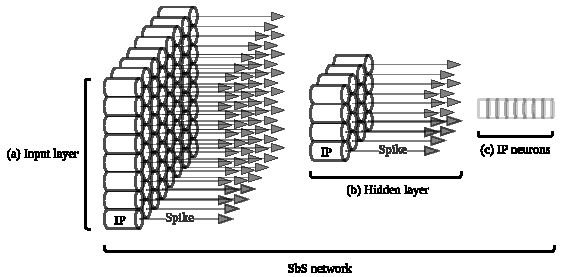
\includegraphics[width=0.5\textwidth]{../figures/SbS_layer.pdf}
	\caption{SbS IPs as independent computational entities, (a) illustrates an input layer with a massive amount of IPs operating as independent computational entities, (b) shows a hidden layer with an arbitrary amount of IPs as independent computational entities, (c) exhibits a set of neurons grouped in an IP.}
	\label{fig:SbS_layer}
\end{figure}


% Fundamentally, SbS is a stochastic gradient descent dynamics
% consistent with Non-Negative Matrix Factorization (NNMF). The stochasticity of gradient descent could
% in principle overcome local minima.  Furthermore, it favors sparse
% solutions with little fluctuations (which is the case for overcomplete
% representations). Finally this specific mechanism for inducing
% sparseness selects those sparse solutions that are robust against
% noise in the inputs.

% In SbS, the expected change at a
% given h-state (i.e. $\Delta h^{s_t}_i 	\propto \left<
% \frac{W(s_t | i) h_i}{\sum_j W(s_t | j) h_j} - 1 \right>_{p(s_t)}$ for all
% $i \in (1,...,N)$ is exactly the same we would have in a low pass
% version of NNMF ($\Delta h_i
% = \sum_s \frac{p(s) W(s | i) h_i}{\sum_j W(s | j) h_j} - 1$). Then,
% for each given h-state, the changes of h induced by SbS consist of the
% expected vector $\Delta h$ plus fluctuations $\eta_i(s_t)$ with
% $<\eta_i(s_t)>p(s_t) = 0$
% (i.e. $\Delta h^{s_t}_i = \sum_s \frac{p(s) W(s | i) h_i}{\sum_j W(s | j) h_j} + \eta_i(s_t)$).
% Thus, SbS performs a random walk with mean $\Delta h$ and some variance, where we have a stochastic process in h-space with the correct
% drift ($\Delta h$) and diffusion. Such processes drift towards states where the drift vanishes except for
% remaining fluctuations. Thus, it produces a Brownian motion
% finally leading to a probability density for h-states centered around
% the fixed point.

% However, even in cases where the problem is convex, NNMF can still have
% manifolds of equivalently optimal solutions. That is, the fixed points
% are not necessarily unique. This is particularly the case for
% overcomplete representations, which can occur when the number of output
% nodes is larger than the number of input nodes. Here, SbS has a tendency
% to select those solutions that have smaller fluctuations of the
% h-values. Simply because h-states with larger fluctuations have a
% smaller probability density in stochastic processes. In the overcomplete
% case these h-vectors are sparse.

% But not only sparseness is favored by SbS, but additionally those among
% the sparse solutions that have the smallest fluctuations. This is the
% famous tornado in the example in the 2008 paper.

\subsection{\REVIEW{Error resilience}}

\REVIEW{To illustrate the error resilience of SbS networks, we present a classification performance under positive additive uniformly distributed noise as external disturbance.} \fig{fig:robustnes_sbs} presents a comparison of the classification performance of an SbS network and a standard \REVIEW{CNN}, with the same amount of
neurons per layer as well as the same layer structure. We trained both neural networks for handwritten digit classification on MNIST dataset\cite{lecun1998mnist} (see \cite{rotermund2019Backpropagation} for details). The figure shows the correctness for the MNIST test set with its $10000$ patterns in dependency of the noise level for positive additive
uniformly distributed noise. The blue curve shows the performance for
the \REVIEW{CNN}, while the red curve shows the performance for
the SbS network with 1200 spikes per inference population. Beginning
with a noise level of 0.1, the respective performances are different
with a p - level of at least $10^{-6}$ (tested with the Fisher exact
test). Increasing the number of spikes per SbS population to 6000
(performance values shown as black stars), shows that more spikes can
improve the performance under noise even more.

\begin{figure}[t!]
	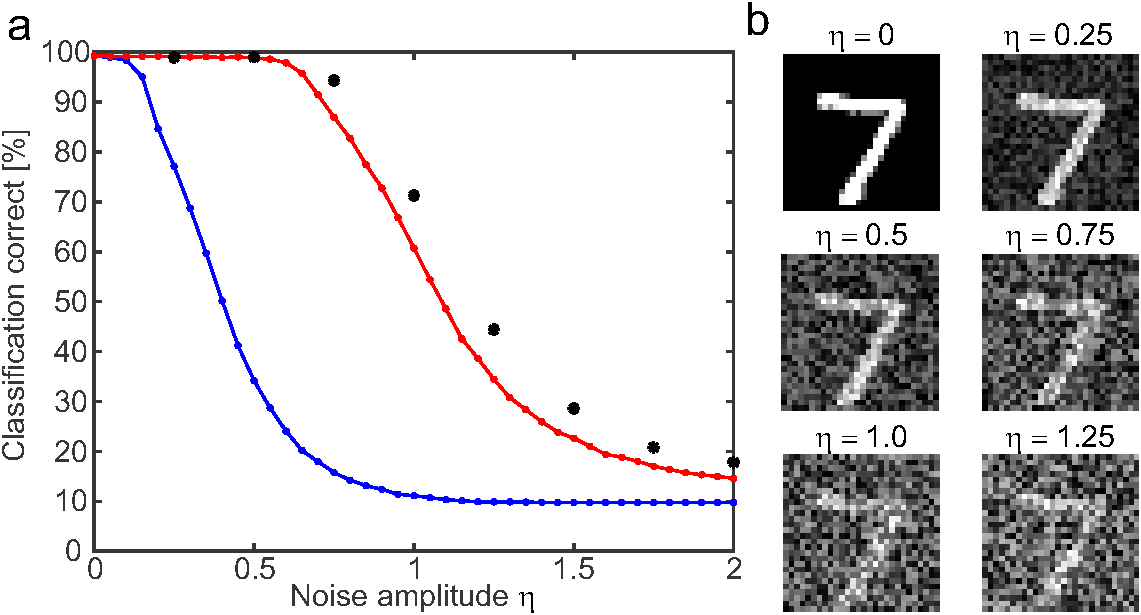
\includegraphics[width=\columnwidth]{../figures/sbs_robustnes.pdf}
	\caption{(a) Performance classification of SbS NN versus equivalent CNN, and (b) example of the first pattern in the MNIST test data set with different amounts of \REVIEW{positive additive uniformly distributed noise}.}
	\label{fig:robustnes_sbs}
\end{figure}



\subsection{Parallelization in SbS networks}
SbS network models are constructed in sequential layered structures, each layer consists of many IPs which can be simulated independently while the communication between the IPs is organized by a low bandwidth signal -- the spikes \cite{Rotermund500280}. Technically, each IP is an independent computational entity (see \fig{fig:SbS_layer}), this allows to design specialized hardware architectures that can be massively parallelized.

\begin{figure}
	\centering
	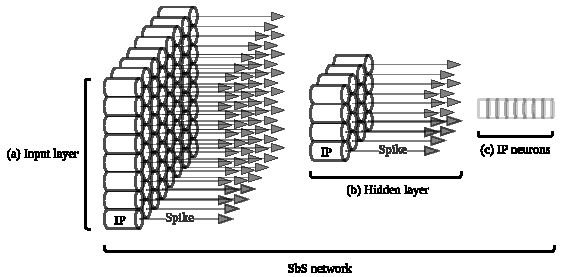
\includegraphics[width=0.5\textwidth]{../figures/SbS_layer.pdf}
	\caption{(a) Illustrates an input layer with a massive amount of IPs operating as independent computational entities. (b) Illustrate a hidden layer with an arbitrary amount of IPs as independent computational entities. (c) Illustrates a set of neurons grouped in an IP. }
	\label{fig:SbS_layer}
\end{figure}